% NoiseMap: prezentácia projektu
% Metódy inžinierskej práce 2026/27, FIIT STU
% Podľa vzoru prezentácie (V. Vranić, J. Lang)
%
% Súbory potrebné na preklad (v tom istom priečinku):
%   diagram.pdf        - vlastný diagram architektúry (zdroj: diagram.tex)
%   esp32_devkitc.jpg  - fotografia: Espressif Systems, dokumentácia ESP-IDF v4.4,
%                        https://github.com/espressif/esp-idf/blob/release/v4.4/docs/_static/esp32-devkitc-functional-overview.jpg
%                        (repozitár ESP-IDF je pod licenciou Apache 2.0)
% Preklad: pdflatex prez_NoiseMap.tex (2x, kvôli prehľadu)

\documentclass{beamer}

%\usetheme{Warsaw}
%\usetheme{Antibes}
\usetheme{JuanLesPins}
%\usetheme{Goettingen}

\usecolortheme{seahorse}
%\usecolortheme{dolphin}
%\usecolortheme{rose}
% https://deic.uab.cat/~iblanes/beamer_gallery/
%\usecolortheme{beaver}

%\useoutertheme[]{sidebar}

\setbeamercovered{transparent}

\usepackage[slovak]{babel}
\usepackage[T1]{fontenc}
\usepackage[utf8]{inputenc}
\usepackage{url}

\usepackage{listings}

\lstset{language=C++,basicstyle=\fontsize{8}{9.6}\selectfont,showstringspaces=false,columns=fullflexible,identifierstyle=\ttfamily,keywordstyle=\bfseries,showstringspaces=false,columns=fullflexible}
% diakritika v komentároch kódu (listings sám nepozná viacbajtové znaky UTF-8)
\lstset{literate=
	{á}{{\'a}}1 {ä}{{\"a}}1 {č}{{\v{c}}}1 {ď}{{\v{d}}}1 {é}{{\'e}}1 {í}{{\'i}}1
	{ľ}{{\v{l}}}1 {ĺ}{{\'l}}1 {ň}{{\v{n}}}1 {ó}{{\'o}}1 {ô}{{\^o}}1 {ŕ}{{\'r}}1
	{š}{{\v{s}}}1 {ť}{{\v{t}}}1 {ú}{{\'u}}1 {ý}{{\'y}}1 {ž}{{\v{z}}}1
	{Č}{{\v{C}}}1 {Š}{{\v{S}}}1 {Ž}{{\v{Z}}}1}

\def\BibTeX{\textsc{Bib}\kern-.08em\TeX}

\newcommand{\footcite}[1]{\footnote{\tiny #1}}
\newcommand{\umlet}{.5}
\newcommand{\emp}[1]{\textit{\alert{#1}}}
\newcommand{\kw}[1]{\mbox{\textbf{#1}}}
\newcommand{\id}[1]{\texttt{#1}}
\newcommand{\stl}{\guillemotleft}
\newcommand{\str}{\guillemotright}

\newcommand{\lsti}{\lstinline[basicstyle=\fontsize{10.5}{12.1}\selectfont]}

\newcommand{\ssection}[1]{
	\section{#1}
	\begin{frame}[fragile=singleslide]\frametitle{}
	\Huge #1
	\end{frame}
}

\newcommand{\ssectionn}[1]{
	\section*{#1}
	\begin{frame}[fragile=singleslide]\frametitle{}
	\Huge #1
	\end{frame}
}

\newenvironment{program}{\begin{beamercolorbox}[rounded=true,shadow=true]{block body}\vspace{-4mm}}{\vspace{-2mm}\end{beamercolorbox}}

\setbeamercolor{fvystup}{fg=white,bg=black}
\newenvironment{vystup}{\begin{beamercolorbox}[rounded=true,shadow=true]{fvystup}}{\end{beamercolorbox}}

\newenvironment{poznamka}{\begin{beamercolorbox}[rounded=true,shadow=false]{block body}}{\end{beamercolorbox}}

\setbeamertemplate{footline}[page number]
{
%\insertpagenumber
%\begin{beamercolorbox}{section in head/foot}
%\vskip2pt\insertnavigation{\paperwidth}\vskip2pt
%\end{beamercolorbox}%
}



\author[Kornilov, Komarchuk, Kholoshyn, Kniaziev]{
	Mykola Kornilov, Danyil Komarchuk,\\
	Kostiantyn Kholoshyn, Valerii Kniaziev}
\institute{
	Fakulta informatiky a informačných technológií\\
	Slovenská technická univerzita v Bratislave}

\subtitle{\vspace{3mm} Metódy inžinierskej práce 2026/2027}

\title[NoiseMap]{NoiseMap: mapovanie hluku v~interiéroch v~reálnom čase
}

\date{\footnotesize 26. október 2026} % upravte na deň prezentácie




\begin{document}

\begin{frame}[fragile=singleslide]
\titlepage
\end{frame}


\begin{frame}[fragile=singleslide]\frametitle{O čom to je}
Keď hľadáme tiché miesto na prácu alebo štúdium, o~skutočnej hlučnosti knižnice, kaviarne či coworkingu sa zvyčajne dozvieme až na mieste.

\bigskip
NoiseMap je návrh platformy, ktorá by zbierala údaje o~hluku vo vnútri budov a~zobrazila ich na interaktívnej mape spolu s~typickým priebehom dňa.

\bigskip
Návštevník by si tak mohol tiché miesto vybrať vopred a~majiteľ budovy by získal prehľad o~tom, kde a~kedy je u~neho hlučno.
\end{frame}


\begin{frame}[fragile=singleslide]\frametitle{Prehľad}
\tableofcontents
\end{frame}


\section{Problém}

\begin{frame}[fragile=singleslide]\frametitle{V čom je problém}
\begin{itemize}
\item Hluk v~budove sa mení
	\begin{itemize}
	\item počas dňa a~týždňa
	\item medzi zónami: tichá zóna, zóna na rozhovor, technická zóna
	\end{itemize}
\item Známe systémy mapujú najmä mestský hluk vo vonkajšom prostredí
	\begin{itemize}
	\item senzorová sieť SONYC v~New Yorku\footcite{J. P. Bello et al. SONYC: A System for Monitoring, Analyzing, and Mitigating Urban Noise Pollution. Communications of the ACM, 62(2):68--77, 2019. \url{https://doi.org/10.1145/3224204}}
	\item participatívne merania mobilom v~projekte NoiseTube\footcite{N. Maisonneuve, M. Stevens, B. Ochab. Participatory noise pollution monitoring using mobile phones. Information Polity, 15:51--71, 2010.}
	\end{itemize}
\item \emp{Interiéry budov zostávajú na mapách hluku prázdnym miestom}
\end{itemize}
\end{frame}


\section{Navrhované riešenie}

\begin{frame}[fragile=singleslide]\frametitle{Dva zdroje údajov}
\begin{itemize}
\item Stacionárne senzorové uzly
	\begin{itemize}
	\item mikrokontrolér ESP32 s~MEMS mikrofónom
	\item inštaluje ich majiteľ budovy, merajú nepretržite
	\end{itemize}
\item Crowdsourcingové merania
	\begin{itemize}
	\item návštevník urobí krátke meranie mobilom
	\item k~meraniu priradí poschodie a~zónu
	\item pokrýva budovy bez senzorov
	\end{itemize}
\item \emp{Surový zvuk neopúšťa zariadenie}: odosiela sa len agregovaná hladina v~dB SPL
\end{itemize}
\end{frame}


\begin{frame}[fragile=singleslide]\frametitle{Senzorový uzol}
\begin{center}
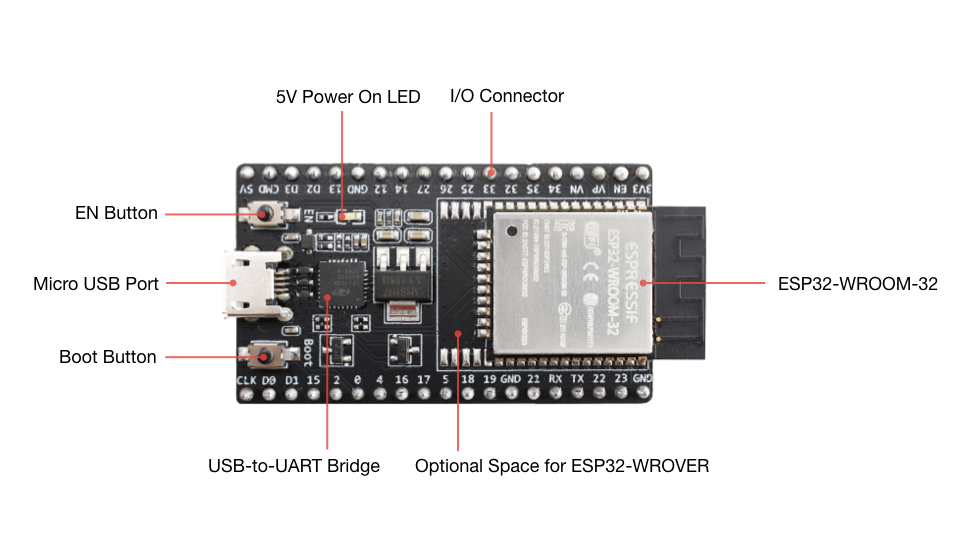
\includegraphics[width=.92\textwidth]{esp32_devkitc.jpg}
\end{center}

{\tiny Vývojová doska ESP32-DevKitC, na ktorej by mohol byť postavený prototyp senzorového uzla. Zdroj: Espressif Systems, dokumentácia ESP-IDF v4.4, \url{https://github.com/espressif/esp-idf/blob/release/v4.4/docs/_static/esp32-devkitc-functional-overview.jpg}}
\end{frame}


\begin{frame}[fragile=singleslide]\frametitle{Architektúra systému}
\begin{center}
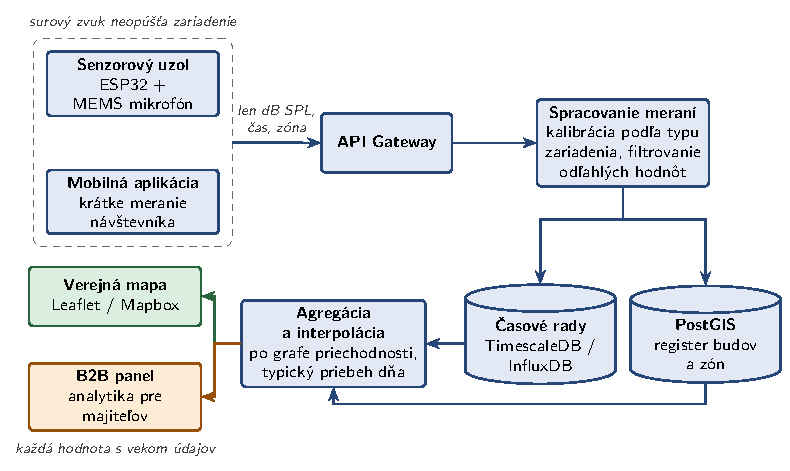
\includegraphics[width=\textwidth]{diagram.pdf}
\end{center}

{\tiny Schematické zobrazenie navrhovanej architektúry (vlastný diagram).}
\end{frame}


\begin{frame}[fragile=singleslide]\frametitle{Výpočet hladiny priamo na zariadení}
\begin{itemize}
\item Z~okna vzoriek sa vypočíta efektívna hodnota (RMS) a~prepočíta sa na dB SPL
\begin{lstlisting}
// jedno okno vzoriek z MEMS mikrofónu (rozhranie I2S)
double hladina_db_spl(const int32_t *vzorky, size_t n) {
   double suma = 0.0;
   for (size_t i = 0; i < n; i++)
      suma += (double)vzorky[i] * vzorky[i];
   double rms  = sqrt(suma / n);
   double dbfs = 20.0 * log10(rms / PLNY_ROZSAH);
   return dbfs + KALIBRACIA_DB;   // posun pre daný typ mikrofónu
}
\end{lstlisting}

\item Konštanta \id{KALIBRACIA\_DB} vychádza z~citlivosti mikrofónu, ktorú uvádza výrobca
\end{itemize}
\end{frame}


\begin{frame}[fragile=singleslide]\frametitle{Čo sa odosiela na server}
\begin{poznamka}
Zariadenie odosiela iba výsledok výpočtu. Zvukový záznam sa neukladá ani neodosiela.
\end{poznamka}

\begin{itemize}
\item Volanie na uzle

\begin{program}
\begin{lstlisting}
odosli(hladina_db_spl(okno, N), cas, zona);
\end{lstlisting}
\end{program}

\item Správa, ktorá príde na server (ilustračný príklad)
\begin{vystup}
\begin{lstlisting}[language={},basicstyle=\ttfamily\fontsize{8}{9.6}\selectfont]
{ "zona":   "kniznica-2p-citaren",
  "db_spl": 47.8,
  "cas":    "2026-10-26T09:15:00Z",
  "zdroj":  "uzol-esp32" }
\end{lstlisting}
\end{vystup}

\end{itemize}
\end{frame}


\section{Spracovanie údajov}

\begin{frame}[fragile=singleslide]\frametitle{Od meraní k mape}
\begin{itemize}
\item Kalibrácia podľa typu zariadenia
	\begin{itemize}
	\item uzly so známou citlivosťou mikrofónu
	\item mobily len s~relatívnou normalizáciou: presnosť aplikácií a~telefónov sa výrazne líši\footcite{C. A. Kardous, P. B. Shaw. Evaluation of smartphone sound measurement applications. Journal of the Acoustical Society of America, 135(4):EL186--EL192, 2014. \url{https://doi.org/10.1121/1.4865269}}
	\end{itemize}
\item Overovanie crowdsourcingu: medián, vylúčenie odľahlých hodnôt, váha podľa dôveryhodnosti
\item Interpolácia so vzdialenosťou po \emph{grafe priechodnosti} miestností, nie vzdušnou čiarou cez steny
\item Typický priebeh dňa z~historických údajov, napr. \uv{ráno ticho, po 17:00 hlučno}
\item \emp{Každá hodnota sa zobrazí s~vekom údajov}
\end{itemize}
\end{frame}


\begin{frame}[fragile=singleslide]\frametitle{Verejná mapa a B2B panel}
\begin{columns}[T]
\begin{column}{.48\textwidth}
\textbf{Verejná mapa}\\[1mm]
{\small pre návštevníkov}
\begin{itemize}
\item tiché miesto v~okolí
\item plán poschodia s~farebnou škálou
\item typický priebeh dňa
\item vek údajov pri každej hodnote
\end{itemize}
\end{column}
\begin{column}{.48\textwidth}
\textbf{B2B panel}\\[1mm]
{\small pre majiteľov budov}
\begin{itemize}
\item hodiny s~najvyšším hlukom
\item porovnanie zón
\item podklady pre akustické úpravy a~zónovanie
\end{itemize}
\end{column}
\end{columns}
\end{frame}


\section{Výzvy}

\begin{frame}[fragile=singleslide]\frametitle{Hlavné výzvy}
\begin{itemize}
\item Nerovnaká presnosť mikrofónov v~mobiloch
\item Dôvera používateľov: aplikácia, ktorá \uv{počúva}, aj keď odosiela len číslo
\item Studený štart: crowdsourcing funguje až pri dostatku meraní v~danom mieste
\item Rozdielne právne pravidlá monitorovania zvuku v~jednotlivých krajinách
\item Zastarávanie jednorazových meraní
\end{itemize}
\end{frame}



\section*{Zhodnotenie a ďalšia práca}
% hviezdička zabezpečí, aby sa táto časť neocitla v prehľade prezentácie

\begin{frame}[fragile=singleslide]\frametitle{Zhodnotenie a ďalšia práca}
\begin{itemize}
\item NoiseMap by spojil senzorové uzly a~merania návštevníkov do jednej mapy hluku v~interiéroch
\item Ochrana súkromia je súčasťou návrhu od začiatku: na server ide len hladina v~dB
\item Ďalej nás čaká
	\begin{itemize}
	\item prehľad literatúry o~kalibrácii a~interpolácii v~interiéroch
	\item prototyp senzorového uzla
	\item návrh overovania crowdsourcingových meraní
	\end{itemize}
\end{itemize}
\end{frame}


\end{document}



Text za príkazom \end{document} LaTeX ignoruje, takže tu možno odkladať slajdy, ktoré zatiaľ nepotrebujeme.
